\documentclass{article}
\usepackage{amsmath, sfmath, multicol, tkz-euclide, array, enumerate, tcolorbox, tabularray}
\renewcommand{\familydefault}{\sfdefault}
\setlength{\parindent}{0cm}
\pagestyle{empty}
\usepackage[left=1in, top=0.5in, right=0.75in, bottom=0.5in]{geometry}
\tcbset{colback=white}

\newcounter{example}[section]
\newenvironment{example}[1][]{\refstepcounter{example}\par\medskip
   {\color{red}\textbf{Example~\theexample. #1}}}{\medskip}

\begin{document}

\section*{Points, Lines, and Planes}

\begin{tcolorbox}[colframe=orange!70!white, coltitle=black, title=\textbf{Today I Can}]
\begin{enumerate}
    \item Understand the basic terms and postulates of geometry.
\end{enumerate}
\end{tcolorbox}

\begin{tcolorbox}[
colframe=black!20!white, 
opacitybacktitle=0.1,
coltitle=black, title=\textbf{Undefined Terms}]
The \textbf{undefined terms} of geometry are \emph{point}, \emph{line}, and \emph{plane}. \newline 

They are considered undefined because we can not give a definition for them without using other geometric terms. We can, at best, describe them.
\end{tcolorbox}

% \begin{center}
% \begin{tabular}{|c|p{0.3\textwidth}|p{0.3\textwidth}|c|}
% \hline
% \textbf{Term}   
% &   \textbf{Description}   
% &   \textbf{Named}  
% &   \textbf{Diagram}    
% \\  \hline
% Point   &
% A location without size.    &
% A dot with a capital letter.    &
% \begin{tikzpicture}
% \tkzDefPoints{0/0/A}
% \tkzDrawPoint[fill=black](A)
% \tkzLabelPoints[right](A)
% \end{tikzpicture}
% \\ \hline
% Line    &
% Straight path that extends in two opposite directions without end. A line contains an infinite number of points.    &
% 2 points with a capital letter, such as $\overleftrightarrow{AB}$ or $\overleftrightarrow{BA}$, or as a single lowercase letter such as $m$.  &
% \begin{tikzpicture}
% \tkzDefPoints{0.5/0/A, 2/0/B}
% \tkzDrawSegment[add = 0.5 and 0.5, <->, >=stealth](A,B)
% \tkzDrawPoints(A,B)
% \tkzLabelPoints[below](A, B)
% \tkzDefPoints{2.7/0/m}    \tkzLabelPoints[right](m)
% \end{tikzpicture}
% \\   \hline  
% Plane   &
% {Flat surface that extends without end. \newline A plane contains infinitely many lines.}   &
% {Capital scripted letter such as $\mathcal{M}$, or by at least 3 points not on the same line such as $ABC$.} &
%     \\  &   &   &
% \raisebox{1cm}{
% \begin{tikzpicture}
% \tkzDefPoints{0/0/W, 2/0/Z, 1/2/X, 3/2/Y}
% \tkzDrawPolygon[fill = yellow!25](W,X,Y,Z)
% \tkzDefPoints{0.5/0.5/A, 1.5/0.75/B, 0.75/1/C}
% \tkzLabelPoints[right](B)
% \tkzLabelPoints[above right](C)
% \tkzLabelPoints[below](A)
% \tkzDrawPoints(A,B,C)
% \tkzLabelPoint[below left](Y){$\mathcal{M}$}
% \end{tikzpicture}}
% \\ \hline
% \end{tabular}
% % \end{center}
% \vspace{0.25in}

\begin{tblr}{|Q[c,m]|Q[c,m,5.75cm]|Q[c,m,5cm]|Q[c,m]|}
\hline
\textbf{Term}   
&   \textbf{Description}   
&   \textbf{Named}  
&   \textbf{Diagram}    
\\  \hline
Point   &
A location without size.    &
A dot with a capital letter.    &
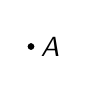
\begin{tikzpicture}
\tkzDefPoints{0/0/A}
\tkzDrawPoint[fill=black](A)
\tkzLabelPoints[right](A)
\end{tikzpicture}
\\ \hline
Line    
&
Straight path that extends in two opposite directions without end. \newline A line contains an infinite number of points.    
&
2 points with a capital letter, such as $\overleftrightarrow{AB}$ or $\overleftrightarrow{BA}$, or as a single lowercase letter such as $m$.  
&
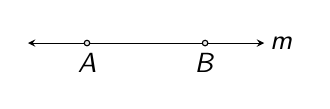
\begin{tikzpicture}
\tkzDefPoints{0.5/0/A, 2/0/B}
\tkzDrawSegment[add = 0.5 and 0.5, <->, >=stealth](A,B)
\tkzDrawPoints(A,B)
\tkzLabelPoints[below](A, B)
\tkzDefPoints{2.7/0/m}    \tkzLabelPoints[right](m)
\end{tikzpicture}
\\   \hline  
Plane   &
Flat surface that extends without end. A plane contains infinitely many lines.
&
Capital scripted letter such as $\mathcal{M}$, or by at least 3 points not on the same line such as $ABC$.
&
\raisebox{-0.65cm}{
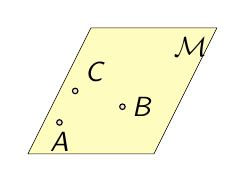
\begin{tikzpicture}[scale=0.8]
\tkzDefPoints{0/0/W, 2/0/Z, 1/2/X, 3/2/Y}
\tkzDrawPolygon[fill = yellow!25](W,X,Y,Z)
\tkzDefPoints{0.5/0.5/A, 1.5/0.75/B, 0.75/1/C}
\tkzLabelPoints[right](B)
\tkzLabelPoints[above right](C)
\tkzLabelPoints[below](A)
\tkzDrawPoints(A,B,C)
\tkzLabelPoint[below left](Y){$\mathcal{M}$}
\end{tikzpicture}}
\\ \hline
\end{tblr}

\vspace{0.25in}

Now that we have the undefined terms above, we can define other geometry vocabulary in terms of them.
\bigskip 

\begin{tcolorbox}[
colframe=black!20!white, 
opacitybacktitle=0.1,
coltitle=black, title=\textbf{Collinear Points}]
Points that lie on the same line.
\end{tcolorbox}

\begin{tcolorbox}[
colframe=black!20!white, 
opacitybacktitle=0.1,
coltitle=black, title=\textbf{Coplanar Points}]
Points and lines that lie on the same plane.
\end{tcolorbox}

\begin{tcolorbox}[
colframe=black!20!white, 
opacitybacktitle=0.1,
coltitle=black, title=\textbf{Space}]
The set of all points in 3 dimensions.
\end{tcolorbox}
% \textbf{Collinear points} are points that lie on the same line. 
% \newline\\

% \textbf{Coplanar points} are points and lines that lie on the same plane. \newline\\

 
% \textbf{Space} is the set of all points in 3 dimensions.
% \newline\\

\begin{example}
Answer each of the following given the diagram shown.
\newline\\
\begin{minipage}{0.6\textwidth}
\begin{enumerate}[(a)]  \setlength{\itemsep}{1cm}
    \item What are two other ways to name $\overleftrightarrow{QT}$?
    \item What are two other ways to name $\mathcal{P}$?
    \item What are the names of 3 collinear points?
    \item What are the names of 4 coplanar points?
\end{enumerate}
\end{minipage}
\hspace{0.55in}
\begin{minipage}{0.30\textwidth}
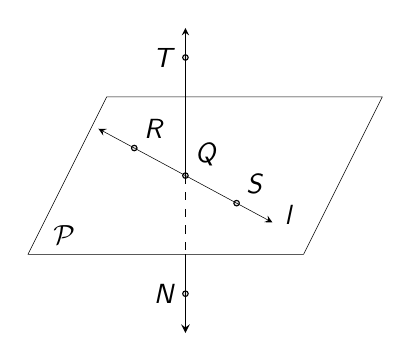
\begin{tikzpicture}
\tkzDefPoints{0/0/A, 3.5/0/B, 1/2/C, 4.5/2/D}
\tkzDrawPolygon(A,B,D,C)
\tkzDefPoints{2/1/Q, 2/-0.5/N, 2/2.5/T, 1.35/1.35/R, 2.65/0.65/S}
\tkzDrawPoints(Q,N,T,R,S)
\tkzLabelPoints[anchor = south west](Q,R,S)
\tkzLabelPoints[left](N,T)
\tkzDrawSegment[add = 0 and 0.25, ->, >=stealth](Q,T)
\draw [dashed](Q) -- (2,0);
\draw [->, >=stealth](2,0) -- (2,-1);
\tkzDrawSegment[add = 0.35 and 0.35, <->, >=stealth](R,S)
\node at (0.2,0) [anchor = south west] {$\mathcal{P}$};
\node at (3.5,0.5) [anchor = east] {$l$};
\end{tikzpicture}
\end{minipage}
\end{example}

\newpage


\setlength{\extrarowheight}{8pt}
\begin{center}
\begin{tblr}{|Q[c,m]|Q[c,m,5.75cm]|Q[c,m,5cm]|Q[c,m]|}
\hline
\textbf{Term}   
&   
\textbf{Description}    
&   
\textbf{Named}  
&   \
\textbf{Diagram}   
\\[3pt] \hline
Segment 
&
Part of a line that contains 2 endpoints and all points in between them.  
&
By 2 endpoints such as $\overline{AB}$ or $\overline{BA}$.    
&
\raisebox{-5pt}{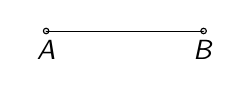
\begin{tikzpicture}
\tkzDefPoints{0/0/A, 2/0/B}
\tkzDrawPoints(A,B)
\tkzLabelPoints[below](A,B)
\tkzDrawSegment(A,B)
\end{tikzpicture}}  \\[8pt] \hline
Ray 
&
Part of a line that consists of 1 endpoint and all the points on the line on one side of the endpoint.
&
By its endpoint and any point on the ray, such as $\overrightarrow{AB}$.
&
\raisebox{-5pt}{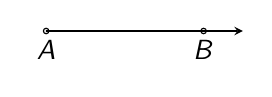
\begin{tikzpicture}
\tkzDefPoints{0/0/A, 2/0/B}
\tkzDrawPoints(A,B)
\tkzLabelPoints[below](A,B)
\draw [->, >=stealth] (A) -- (2.5,0);
\end{tikzpicture}}
\\[8pt] \hline
Opposite Rays
&
2 rays that share an endpoint and form a line.
&
By their shared endpoint and any point on each ray such as $\overrightarrow{CA}$ or $\overrightarrow{CB}$.
&
\raisebox{-5pt}{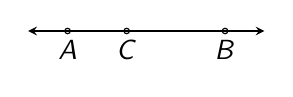
\begin{tikzpicture}
\tkzDefPoints{0/0/A, 2/0/B, 0.75/0/C}
\tkzDrawPoints(A,B,C)
\tkzLabelPoints[below](A,B,C)
\draw [<->, >=stealth] (-0.5,0) -- (2.5,0);
\end{tikzpicture}}
\\[8pt] \hline
\end{tblr}
\end{center}
\vspace{0.25in}

\begin{example}
Answer each of the following given the diagram shown. \bigskip 

\begin{minipage}{0.5\textwidth}
\begin{enumerate}[(a)]  \setlength{\itemsep}{1.5cm}
    \item What are the names of the segments in the figure?
    \item What are the names of the rays in the figure?
    \item Which of the rays in part (b) are opposite rays?
\end{enumerate}
\end{minipage}
\hspace{0.5in}
\begin{minipage}{0.4\textwidth}
\begin{tikzpicture}[rotate = 30]
\tkzDefPoints{0/0/D, 2/0/E, 3.5/0/F}
\tkzDrawPoints(D,E,F)
\tkzLabelPoints[below](D,E,F)
\tkzDrawSegment[add = 0.15 and 0.15, <->, >=stealth](D,F)
\end{tikzpicture}
\end{minipage}
\end{example}
\vspace{1in}

\begin{tcolorbox}[
colframe=black!20!white, 
opacitybacktitle=0.1,
coltitle=black, title=\textbf{Postulate (a.k.a. Axiom)}]
An accepted statement of fact.
\end{tcolorbox}
\vspace{0.5in}


\textbf{Some Geometry Postulates:}
\begin{itemize}
    \item Through any two points there is a line.
    \item If 2 different lines intersect, they intersect at a point.
    \item If 2 different planes intersect, they intersect at a line.
    \item You can draw a plane through any 3 noncollinear points.
\end{itemize}

\newpage 

\begin{example}
Each surface of the box represents a plane. What is the intersection of plane $ADC$ and plane $BFG$? \newline 

\emph{Note:} The dashed line segments represent segments you could not see if the figure was constructed in our 3-dimensional space. \bigskip 

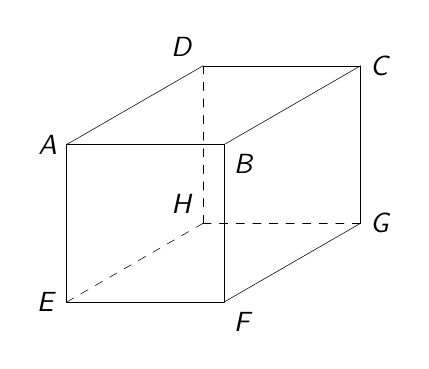
\begin{tikzpicture}
\tkzDefPoints{0/0/E, 2/0/F, 2/2/B, 0/2/A}
\tkzDrawPolygon(E,F,B,A)
\tkzDefShiftPoint[A](30:2){D}
\tkzDefShiftPoint[B](30:2){C}
\tkzDefShiftPoint[E](30:2){H}
\tkzDefShiftPoint[F](30:2){G}
\tkzDrawSegments(A,D B,C F,G D,C G,C)
\tkzDrawSegments[dashed](E,H H,D H,G)
\tkzLabelPoints[left](A,E)
\tkzLabelPoints[above left](D,H)
\tkzLabelPoints[right](G,C)
\tkzLabelPoints[below right](B,F)
\end{tikzpicture}
\end{example} 
\vspace{0.25in}


When naming planes with 4 or more points, list the points in order either clockwise or counterclockwise.

\vspace{0.25in}

\begin{example} Use the figure to answer each. \bigskip 

\begin{enumerate}[(a)]
\item What plane contains $N$, $P$, and $Q$? Shade it.

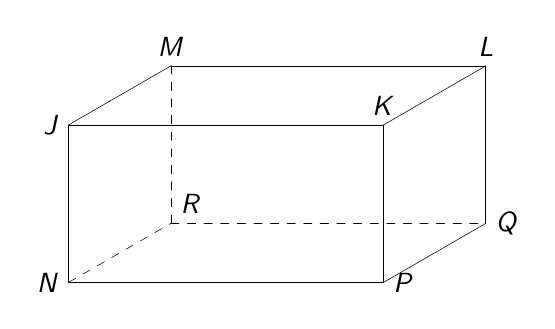
\begin{tikzpicture}
\tkzDefPoints{0/0/N, 4/0/P, 4/2/K, 0/2/J}
\tkzDrawPolygon(N,P,K,J)
\tkzDefShiftPoint[N](30:1.5){R}
\tkzDefShiftPoint[J](30:1.5){M}
\tkzDefShiftPoint[K](30:1.5){L}
\tkzDefShiftPoint[P](30:1.5){Q}
\tkzDrawSegments[dashed](N,R R,M R,Q)
\tkzDrawSegments(J,M M,L L,K L,Q Q,P)
\tkzLabelPoints[left](J,N)
\tkzLabelPoints[above](M,K,L)
\tkzLabelPoints[above right](R)
\tkzLabelPoints[right](P,Q)
\end{tikzpicture}

\vspace{1in}

\item What plane contains $J$, $M$, and $Q$? Shade it.

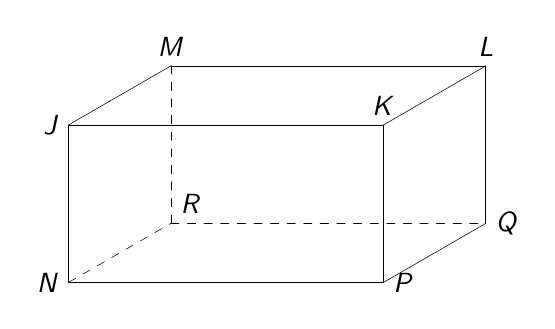
\begin{tikzpicture}
\tkzDefPoints{0/0/N, 4/0/P, 4/2/K, 0/2/J}
\tkzDrawPolygon(N,P,K,J)
\tkzDefShiftPoint[N](30:1.5){R}
\tkzDefShiftPoint[J](30:1.5){M}
\tkzDefShiftPoint[K](30:1.5){L}
\tkzDefShiftPoint[P](30:1.5){Q}
\tkzDrawSegments[dashed](N,R R,M R,Q)
\tkzDrawSegments(J,M M,L L,K L,Q Q,P)
\tkzLabelPoints[left](J,N)
\tkzLabelPoints[above](M,K,L)
\tkzLabelPoints[above right](R)
\tkzLabelPoints[right](P,Q)
\end{tikzpicture}
\end{enumerate}
\end{example}

\end{document}
